% Options for packages loaded elsewhere
\PassOptionsToPackage{unicode}{hyperref}
\PassOptionsToPackage{hyphens}{url}
%
\documentclass[
]{article}
\usepackage{lmodern}
\usepackage{amssymb,amsmath}
\usepackage{ifxetex,ifluatex}
\ifnum 0\ifxetex 1\fi\ifluatex 1\fi=0 % if pdftex
  \usepackage[T1]{fontenc}
  \usepackage[utf8]{inputenc}
  \usepackage{textcomp} % provide euro and other symbols
\else % if luatex or xetex
  \usepackage{unicode-math}
  \defaultfontfeatures{Scale=MatchLowercase}
  \defaultfontfeatures[\rmfamily]{Ligatures=TeX,Scale=1}
\fi
% Use upquote if available, for straight quotes in verbatim environments
\IfFileExists{upquote.sty}{\usepackage{upquote}}{}
\IfFileExists{microtype.sty}{% use microtype if available
  \usepackage[]{microtype}
  \UseMicrotypeSet[protrusion]{basicmath} % disable protrusion for tt fonts
}{}
\makeatletter
\@ifundefined{KOMAClassName}{% if non-KOMA class
  \IfFileExists{parskip.sty}{%
    \usepackage{parskip}
  }{% else
    \setlength{\parindent}{0pt}
    \setlength{\parskip}{6pt plus 2pt minus 1pt}}
}{% if KOMA class
  \KOMAoptions{parskip=half}}
\makeatother
\usepackage{xcolor}
\IfFileExists{xurl.sty}{\usepackage{xurl}}{} % add URL line breaks if available
\IfFileExists{bookmark.sty}{\usepackage{bookmark}}{\usepackage{hyperref}}
\hypersetup{
  pdftitle={Analiza połączeń lotniczych w Europie pod kątem rozprzestrzeniania epidemii},
  pdfauthor={Wojciech Agaciński},
  hidelinks,
  pdfcreator={LaTeX via pandoc}}
\urlstyle{same} % disable monospaced font for URLs
\usepackage[margin=1in]{geometry}
\usepackage{longtable,booktabs}
% Correct order of tables after \paragraph or \subparagraph
\usepackage{etoolbox}
\makeatletter
\patchcmd\longtable{\par}{\if@noskipsec\mbox{}\fi\par}{}{}
\makeatother
% Allow footnotes in longtable head/foot
\IfFileExists{footnotehyper.sty}{\usepackage{footnotehyper}}{\usepackage{footnote}}
\makesavenoteenv{longtable}
\usepackage{graphicx,grffile}
\makeatletter
\def\maxwidth{\ifdim\Gin@nat@width>\linewidth\linewidth\else\Gin@nat@width\fi}
\def\maxheight{\ifdim\Gin@nat@height>\textheight\textheight\else\Gin@nat@height\fi}
\makeatother
% Scale images if necessary, so that they will not overflow the page
% margins by default, and it is still possible to overwrite the defaults
% using explicit options in \includegraphics[width, height, ...]{}
\setkeys{Gin}{width=\maxwidth,height=\maxheight,keepaspectratio}
% Set default figure placement to htbp
\makeatletter
\def\fps@figure{htbp}
\makeatother
\setlength{\emergencystretch}{3em} % prevent overfull lines
\providecommand{\tightlist}{%
  \setlength{\itemsep}{0pt}\setlength{\parskip}{0pt}}
\setcounter{secnumdepth}{-\maxdimen} % remove section numbering
% https://github.com/rstudio/rmarkdown/issues/337
\let\rmarkdownfootnote\footnote%
\def\footnote{\protect\rmarkdownfootnote}

% https://github.com/rstudio/rmarkdown/pull/252
\usepackage{titling}
\setlength{\droptitle}{-2em}

\pretitle{\vspace{\droptitle}\centering\huge}
\posttitle{\par}

\preauthor{\centering\large\emph}
\postauthor{\par}

\predate{\centering\large\emph}
\postdate{\par}

\title{Analiza połączeń lotniczych w Europie pod kątem rozprzestrzeniania
epidemii}
\author{Wojciech Agaciński}
\date{2.2.2020}

\begin{document}
\maketitle

\hypertarget{cel-projektu}{%
\section{Cel projektu}\label{cel-projektu}}

Celem niniejszego projektu jest analiza sieci połączeń lotniczych w
Europie, pod kątem potencjanego rozprzestrzeniania się chorób zakaźnych.
Jak wiadomo, transport lotniczny jest jednym z najpopularniejszych metod
transportu masowego na świecie. Z uwagi na najmniejszy czas podróży
wśród wszystkich innych metod, rozbudowaną sieć oraz ogromną liczbę
pasażeróW, transport lotniczy może stanowić poważne zagrożenie w
kontekście transmisji chorób zakaźnych.

Inspiracją niniejszego projektu jest trwająca epidemia koronawirusa
(2019-nCoV), która rozpoczęła się w mieście Wuhan pod koniec 2019 roku.
Projekt ma na celu próbę odpowiedzania na dwa pytania: które z lotnisk w
Europie są najbardziej narażone na dalsze rozprzestrzenianie
chorobotwórczych patogenów, oraz które lotniska mogą stać się dalszymi
celami, gdy dojdzie już do infekcji na kontynencie.

\hypertarget{informacje-o-zbiorze-danym}{%
\section{Informacje o zbiorze danym}\label{informacje-o-zbiorze-danym}}

Analizie został poddany zbiór danych ``EU-AIR TRANSPORTATION
MULTIPLEX'', dostępny pod adresem
\url{https://comunelab.fbk.eu/data.php}. Zawiera on sieć połączeń
pomiędzy lotniskami w Europie. Dodatkowo, podzielony został na wartswy
odpowiadające różnym liniom lotniczym.

\hypertarget{podstawowe-informacje-na-temat-zbioru}{%
\subsection{Podstawowe informacje na temat
zbioru}\label{podstawowe-informacje-na-temat-zbioru}}

\begin{verbatim}
## [1] " Liczba wierzchołków (lotnisk):  450"
\end{verbatim}

\begin{verbatim}
## [1] " Liczba krawędzi (połączeń):  3588"
\end{verbatim}

\hypertarget{struktura-danych}{%
\subsection{Struktura danych}\label{struktura-danych}}

Informacje na temat wierzchołków sieci - zawarte w pliku
``EUAirTransportation\_nodes.txt''. Jest to w zasadzie słownik
metadanych, zawierający nazwy oraz koordynaty lotnisk.

\begin{longtable}[]{@{}rlrr@{}}
\toprule
nodeID & nodeLabel & nodeLong & nodeLat\tabularnewline
\midrule
\endhead
1 & LCLK & 33.630278 & 34.87889\tabularnewline
2 & EDDF & 8.570555 & 50.03333\tabularnewline
3 & EDDK & 7.142779 & 50.86583\tabularnewline
4 & EGNX & -1.328055 & 52.83111\tabularnewline
5 & EGTE & -3.413888 & 50.73444\tabularnewline
6 & LTBJ & 27.155001 & 38.28917\tabularnewline
\bottomrule
\end{longtable}

Informacje na temat krawędzi sieci - zawarte w pliku
``EUAirTransportation\_multiplex.edges''. Jest to właściwy opis topologi
opisywanej sieci, na podstawie której konstruowany jest graf.

\begin{longtable}[]{@{}rrrr@{}}
\toprule
V1 & V2 & V3 & V4\tabularnewline
\midrule
\endhead
1 & 1 & 2 & 1\tabularnewline
1 & 1 & 38 & 1\tabularnewline
1 & 2 & 7 & 1\tabularnewline
1 & 2 & 8 & 1\tabularnewline
1 & 2 & 10 & 1\tabularnewline
1 & 2 & 14 & 1\tabularnewline
\bottomrule
\end{longtable}

\hypertarget{informacje-na-temat-sieci}{%
\subsection{Informacje na temat sieci}\label{informacje-na-temat-sieci}}

\hypertarget{rozkux142ad-stopni-wejux15bciowych}{%
\subsubsection{Rozkład stopni
wejściowych}\label{rozkux142ad-stopni-wejux15bciowych}}

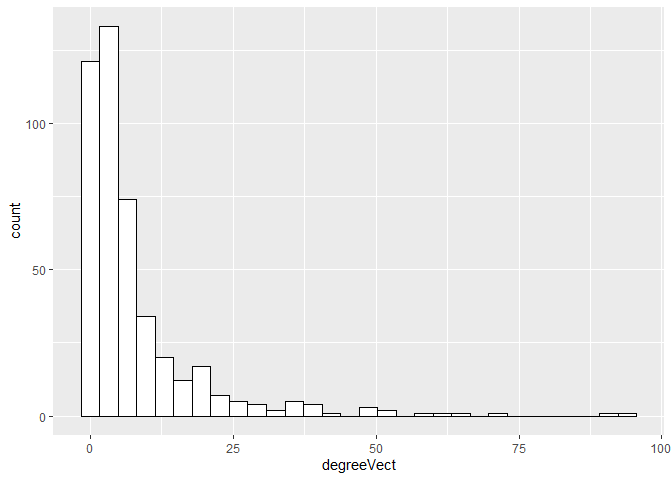
\includegraphics{README_files/figure-latex/unnamed-chunk-5-1.pdf}

\hypertarget{rozkux142ad-stopni-wyjux15bciowych}{%
\subsubsection{Rozkład stopni
wyjściowych}\label{rozkux142ad-stopni-wyjux15bciowych}}

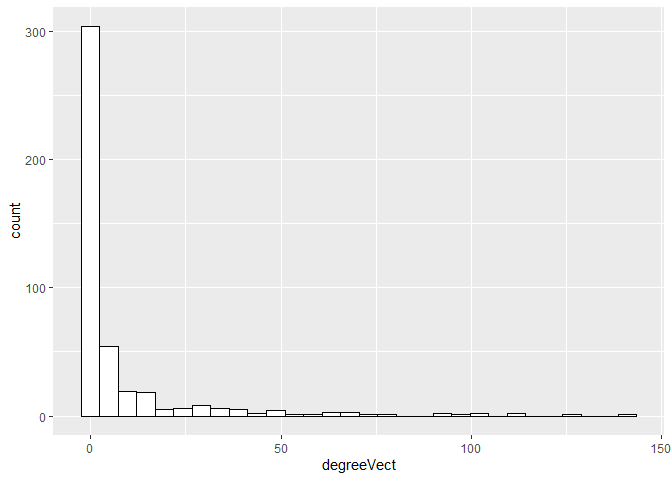
\includegraphics{README_files/figure-latex/unnamed-chunk-6-1.pdf}

\hypertarget{rozkux142ad-dux142ugoux15bci-najkruxf3tszych-ux15bcieux17cek}{%
\subsubsection{Rozkład długości najkrótszych
ścieżek}\label{rozkux142ad-dux142ugoux15bci-najkruxf3tszych-ux15bcieux17cek}}

Przykładowe najkrótsze ścieżki pomiędzy parami wybranych lotnisk

\begin{longtable}[]{@{}lrrrrr@{}}
\toprule
& LTBJ & LFPG & LFBO & EGNT & EDDP\tabularnewline
\midrule
\endhead
LCLK & 2 & 2 & 2 & 2 & 2\tabularnewline
EDDF & 1 & 1 & 1 & 2 & 1\tabularnewline
EDDK & 1 & 1 & 2 & 2 & 1\tabularnewline
EGNX & 2 & 1 & 2 & 2 & 1\tabularnewline
EGTE & 2 & 1 & 2 & 1 & 2\tabularnewline
\bottomrule
\end{longtable}

\hypertarget{poux15brednictwo}{%
\subsubsection{Pośrednictwo}\label{poux15brednictwo}}

\begin{verbatim}
## [1] 0.3035204
\end{verbatim}

\hypertarget{lokalny-wspuxf3ux142czynnik-gronowania}{%
\subsubsection{Lokalny współczynnik
gronowania}\label{lokalny-wspuxf3ux142czynnik-gronowania}}

\begin{verbatim}
## [1] 0.5054187
\end{verbatim}

\hypertarget{miary-oceny-sieci}{%
\subsubsection{Miary oceny sieci}\label{miary-oceny-sieci}}

Gęstość

\begin{verbatim}
## [1] 0.01775798
\end{verbatim}

Średnia bliskość

\begin{verbatim}
## [1] 7.653067e-06
\end{verbatim}

Promień

\begin{verbatim}
## [1] 0
\end{verbatim}

\hypertarget{wizualizacja-sieci}{%
\section{Wizualizacja sieci}\label{wizualizacja-sieci}}

Po wczytaniu niezbędnych danych, tworzony jest graf, zawierający w
atrybutach informacje o współrzędnych geograficznych lotnisk. Jest to
istotne przy tworzeniu wizualizacji sieci. Identyfikatory wierzchołków,
pomiędzy którymi znajdują się opisywane w głównym pliku krawędzie, są
mapowane na nazwy, a właściwie skróty określajace lotniska. Poniżej
znajduje graficzna repezentacja sieci.

\hypertarget{wizualizacja-lotnisk-z-koordynatami}{%
\subsection{Wizualizacja lotnisk z
koordynatami}\label{wizualizacja-lotnisk-z-koordynatami}}

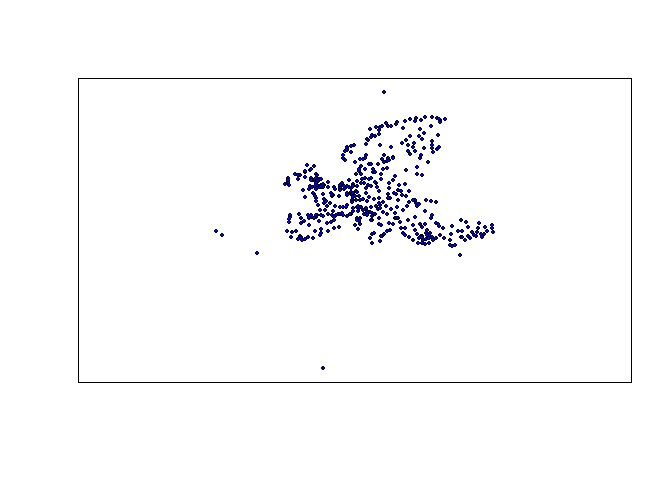
\includegraphics{README_files/figure-latex/unnamed-chunk-13-1.pdf}

\hypertarget{wizualizacja-poux142ux105czeux144}{%
\subsection{Wizualizacja
połączeń}\label{wizualizacja-poux142ux105czeux144}}

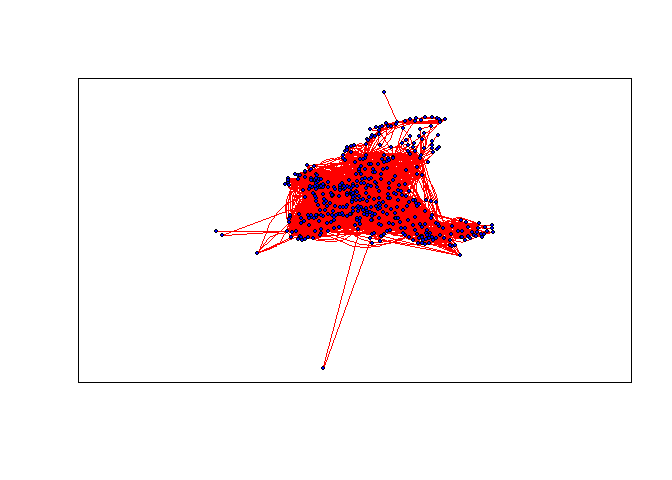
\includegraphics{README_files/figure-latex/unnamed-chunk-14-1.pdf}

\hypertarget{najbardziej-naraux17cone-lotniska}{%
\section{Najbardziej narażone
lotniska}\label{najbardziej-naraux17cone-lotniska}}

W przypadku wybuchu epidemii, bardzo ważnym działaniem jest zapobieganie
powstawaniu kolejnych ognisk choroby. Jedna chora osoba jest wstanie
zainfekować dzięsiątki innych, a dodatkowo, jeżeli odbędzie się to
podczas podroży, może to rozprzestrzenić chorobę pomięDzy różnymi
krajami, a nawet kontynentami. Aby prewencja była skuteczka, warto by
było oszacować najbardziej narażone punkty, w których szansa na
pojawienie się osoby zarażonej jest największa.

W przypadku naszej analizy, jednym z podejść byłoby wyznaczenie lotnisk,
które obsługuje najwięcej różnych połączeń. Takie lotnisko, będąc hubem,
mogłoby obsługiwać zarażonych pasażerów z wielu kierunków. Przyjrzyjmy
się które lotniska spełniają to kryterium - wykorzystamy do tego stopnie
wejściowe wierzchołków.

\begin{verbatim}
## [1] "EHAM" "EDDF" "EGSS" "LFPG" "LEMD"
\end{verbatim}

\hypertarget{strategia-zapobiegania-dalszym-infekcjom}{%
\section{Strategia zapobiegania dalszym
infekcjom}\label{strategia-zapobiegania-dalszym-infekcjom}}

\end{document}
